% This is samplepaper.tex, a sample chapter demonstrating the
% LLNCS macro package for Springer Computer Science proceedings;
% Version 2.20 of 2017/10/04
%
\documentclass[runningheads]{llncs}
%
\usepackage{graphicx}
% Add assets folder to path for images. 
\graphicspath{{assets/}}

\usepackage{amsmath,amssymb,float,url}

% Hide red underlines for URLs. 
\usepackage[hidelinks]{hyperref}

% Stack two figures on top of each other.
\usepackage{subcaption}

% Make caption text font smaller.
\usepackage{caption}
\captionsetup[figure]{font=small,labelfont=small}
% Make table-caption gap larger (source: https://bit.ly/3zm0wRn)
\captionsetup[table]{skip=10pt}

% Used for displaying a sample figure. If possible, figure files should
% be included in EPS format.
%
% If you use the hyperref package, please uncomment the following line
% to display URLs in blue roman font according to Springer's eBook style:
% \renewcommand\UrlFont{\color{blue}\rmfamily}

\begin{document}
%
\title{Machine Learning for Fish Oil Analysis \thanks{Supported by organization Plant and Food Research.}}
%
%\titlerunning{Abbreviated paper title}
% If the paper title is too long for the running head, you can set
% an abbreviated paper title here
%
\author{Jesse Wood\inst{1}\orcidID{0000-1111-2222-3333} \and
  Bach Hoai Nguyen\inst{1}\orcidID{1111-2222-3333-4444} \and
  Bing Xue\inst{1}\orcidID{2222--3333-4444-5555} \and 
  Mengjie Zhang\inst{1}\orcidID{2222--3333-4444-5555} \and 
  Daniel Killeen\inst{2}\orcidID{2222--3333-4444-5555}
}
%
\authorrunning{J. Wood et al.}
% First names are abbreviated in the running head.
% If there are more than two authors, 'et al.' is used.
%
\institute{Victoria University of Wellington, Te Herenge Waka, PO Box 600, Wellington 6140, New Zealand\\
  \email{jesse.wood@ecs.vuw.ac.nz}\\
  \email{bach.nguyen@ecs.vuw.ac.nz}\\
  \email{bing.xue@ecs.vuw.ac.nz}\\
  \email{mengjie.zhang@ecs.vuw.ac.nz}\\ 
  \and 
  Plant and Food Research, Port Nelson, Nelson 7010, New Zealand\\
  \email{Daniel.Killeen@plantandfood.co.nz}\\
}

%
\maketitle              % typeset the header of the contribution
%
\begin{abstract}
  % The abstract should briefly summarize the contents of the paper in
  % 150--250 words.
  
  Gas chromatography (GC) can be used to identify chemical compounds present within tissue samples for quality assurance in food science.
  Existing analytical chemistry techniques for processing GC data are manual and time-consuming.
  Here, we explore classification algorithms for fish oil data that automate and significantly reduce the time required to process GC data.
  We find the Linear SVC model can predict the fish species with near-perfect accuracy.
  Visualisation is used to explore the interpretability of the models such that their efficacy can be verified for use in a factory setting.
  The fish oil data is high-dimensional and low sample size.
  We compare state-of-the-art feature selection methods to reduce the dimensionality of the data.
  High accuracy is possible with very few features for the MRMR and ReliefF feature selection methods.
  
  \keywords{Feature Selection  \and Gas Chromatography \and Support Vector Machines \and Food Science}
\end{abstract}
%
%
%


\section{Introduction}

% \begin{itemize}
%     \item Introduce fish oil analysis: what it is, why it is important. 
%     \item Narrowing down to fish classification as an essential step: fish types, fish parts. 
%     \item Existing limitations of fish classification: manually, labour intensive. 
%     \item How machine learning can be used to address the above limitations. 
% \end{itemize}

Gas chromatography \cite{eder1995gas} is an chemistry technique we use to analyze fish oils. 
It can determine the structure of chemical compounds present in a given sample \cite{restek2018high}. 
This is important for quality assurance in a factory setting, especially in food science. 
We want to be confident that our food labels are accurate and reduce/eliminate cross contamination between different food products. 
To identify cross-contanimation we use fish classification. 
Given a fish oil sample, we can identify the fish species (i.e. Bluecod, Tarakihi), and part (Head, Fins).
The existing techniques for performing fish classification are time consuming and laborious. 
Chemists compare a given sample to reference samples to determine which class it likely belongs to. 
Previous work on gas chromatrography \cite{bi2020gc,matyushin2020gas}, has shown machine learning can be used to automate classification. 

In this paper we explore machine learning techniques to automate the process of identifying fish species and part on GC data. 
Firstly, classifications algorithms are evaluated for their ability to determine the fish species and part. 
Visualisation is used to explore the interpretability of successful models.
It is important to verify their efficacy with domain knowledge before these algorithms can be deployed in a real-world setting.
Secondly, feature selection is used to eliminate redundant features, whilst maintaining high-accuracy predictions. 

Specifically, our work is divided into two main sections: 
\begin{enumerate}
  \item Classification Algorithms
  \item Feature Selection
  \item Visualisation
\end{enumerate}

\section{Background}

This paper is a multi-disciplnary effort.
Domain expertise in chemistry and machine learning is required to extract knowledge from the fish oil data. 
Before we explore the data, here we provide domain knowlegde required to undertsand this paper. 

Specially, the background covers: 
\begin{enumerate}
  \item Chromatrography methods: how the raw fish oil data is collected.
  \item Classification algorithms: introduce classification algorithms used in the paper.
  \item Feature selection: main concepts.
\end{enumerate}

\subsection{Gas Chromatorgraphy}

Gas chromatography (GC) is a technique for the analysis of chemical compounds \cite{eder1995gas,restek2018high,khan2013gas}.
The process sperates compounds based on their bioling point and molecular weight.
A compound is injected as a liquid, then heat is applied to vaporize it into a gas. 
A bioling point is a termparture which it changes phase, from liquid to gas. 
This process is referred to as a phase transition. 
The speed at which a compound is vaporized dpeends on its bioling point. 
The vaporized gases travel through a long couild tube.
That tube has a detector at the end, this detects the rate and inesity which compounds reach the tube's end. 

\begin{figure}[htb]
  \centering
  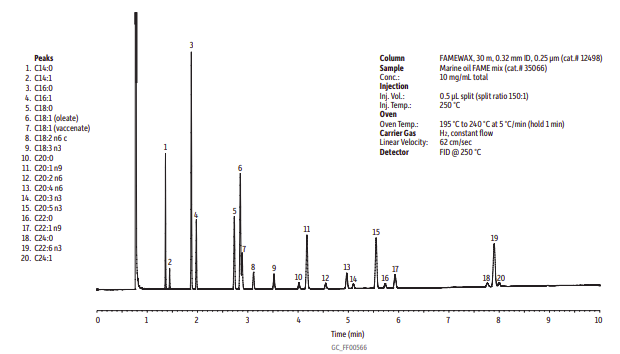
\includegraphics[width=8.5cm]{chromatograph.png}
  \caption{
    Gas chromatograph: the artifact of the GC method \cite{restek2018high}.
    The detection is used to visualize intensity (y) and time (x) on a chromotrogaph.}
  \label{fig:gas-chromatography}% Hide red underlines for URLs. 
  \captionsetup[figure]{font=small,labelfont=small}
\end{figure}

Chemists use the chromatograms of known compounds as a reference when classifying new ones.
Take a known example, say \emph{methyl eladiate}.
We compare this reference sample to an unknown sample.
Analysis can infer the unknown compound since they share the same peaks as the known one.
GC is not a definitive technique \cite{khan2013gas}, so it is often used in conjunction with other techniques.
Mass spectrometry is one such technique \cite{restek2018high}.

The existing task of classifying chemical compounds based on a chromatograph is laborious \cite{eder1995gas,restek2018high}.
The spikes on the graph represent peaks.
Each peak represents a resolved chemical compound.
Chemists integrate the area under each peak, and compare this to a reference sample, to classify the compound.
GC must be performed slowly to ensure that the peaks are not too broad.
This ensures each peak resolves and represents a single compound.
Once we know what compounds are present in a sample it becomes possible to identify what the sample is.
For this fish oil data, we classify a sample into two categories:

\begin{enumerate}
  \item Species
  \item Part
\end{enumerate}

Using machine learning techniques it may be possible to speed the process up.
Machine learning algorithms identify patterns in the data.
These patterns can be used to classify the sample efficiently.
An interpretable and accurate model has the potential to be deployed in a factory setting.
It would eliminate the need for manual work.
Additionally, an algorithm that can classify unresolved peaks would have an impact on the chemistry field.
This increases the speed at which GC is performed, increasing the volumetric efficiency of the production line \cite{musk2020battery}.

\subsection{Classification Algorithms}

The classification task is to identify the class label for an instance from the dataset.
We perform two classification tasks and measure their performance:

\begin{enumerate}
  \item Species: Identify the species of fish (i.e. Bluecod).
  \item Part: Identify the part of the fish (i.e. Head).
\end{enumerate}

A supervised learning method creates a model from a labelled dataset - the train set.
We measure the ability of the model to generalize on unseen data - the test set.
We give the model a tissue sample from a fish.
Based on what it has learnt, it predicts the species and part for that fish.
The existing analytical chemistry techniques for performing this task are laborious and time-consuming.
We desire a model that is interpretable and has high predictive accuracy.
We can then use the model to automate this task.
Thus, it has real-world applications for quality assurance in a factory setting.

\subsubsection{Support Vector Machines}
\label{sec:background-svm}

Cortes and Vapnik proposed the Support Vector Machine (SVM) \cite{cortes1995support}.
This model creates a hyperplane that can draw distinct class boundaries between classes.
We call these class boundaries the support vectors.
We are performing multi-class classification, so it used a one-vs-all approach \cite{sklearn2021feature}.
This creates a divide between one class and the rest, then repeats for the other classes.

\subsubsection{Model}
\label{sec:background-svm-model}

The sklearn library provides several SVM models for classification.
The default model uses the RBF kernel.
Other models use different kernels and parameters \cite{sklearn2021feature}.
Some models remove trainable parameters.
Instead, the user can set the number of support vectors \cite{scholkopf2000new}.

\subsubsection{Kernel}
\label{sec:background-svm-kernel}

The model requires a kernel function.
This determines the shape of the support vectors in the hyperplane.
Different kernels capture data of varying complexities.
The original hyperplane algorithm used a linear kernel \cite{aizerman1964theoretical}.
Later, non-linear kernels we introduced.
These employ the kernel trick \cite{boser1992training}.
Figure~\ref{fig:kernels} shows support vectors for each kernel on a 2D plane.
This provides an intuition for each kernel.

\begin{figure}[htb]
  \centering
  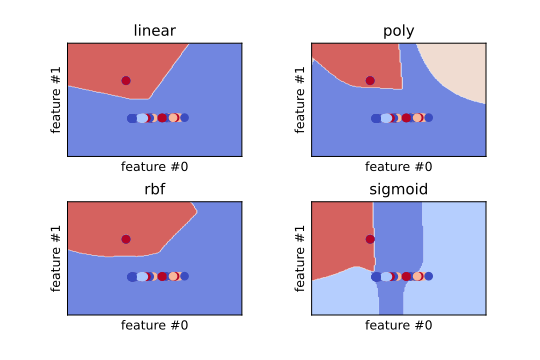
\includegraphics[width=8.5cm]{kernels.png}
  \caption{
    SVM kernels shapes are shown.
    Specifically, linear, polynomial, radial basis function (rbf) and sigmoidal kernal are shown.}
  \label{fig:kernels}
\end{figure}

\subsubsection{Hyperplane Coefficients}
\label{sec:background-svm-hyperplane}

The l1 regularization term leads to sparse models.
So, they include fewer features - making them easier to interpret.
Eq~\ref{eq:hyperplane} defines the total hyperplane as

\begin{align}\label{eq:hyperplane}
  \beta_{\text{t}} = \text{minmax}(
  \sum_{\text{c} \in \text{C}}
  |\beta_{\text{c}}|
  )
\end{align}

where there is the number of classes ($c \in C$) sets of hyperplane coefficients.
$\beta_{\text{t}}$ coefficient as the sum of hyperplane coefficients magnitude for each class $\beta_{\text{c}}$.
We normalize the coefficients with a min-max feature scaling.
The total hyperplane for both datasets is given in Figure~\ref{fig:hyperplane-coefficients}.

\begin{figure}[htb]
  \centering  
  \begin{subfigure}[b]{.45\linewidth}
    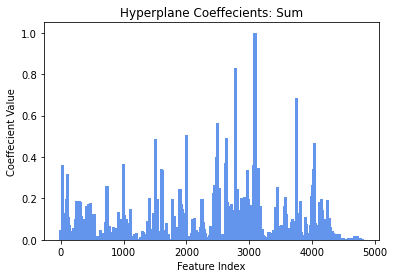
\includegraphics[width=\linewidth]{fish_total_coefficients.png}
    \caption{Fish Species: Hyperplane Coefficients}\label{fig:fish-hyperplane-coeffcients}
  \end{subfigure}
  \begin{subfigure}[b]{.45\linewidth}
    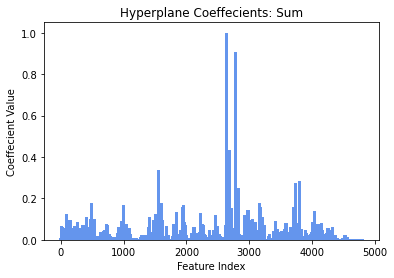
\includegraphics[width=\linewidth]{part_total_coefficients.png}
    \caption{Fish Part: Hyperplane Coefficients}\label{fig:part-hyperplane-coeffcients}
  \end{subfigure}
  \caption[Two numerical solutions]{
    Hyperplane coefficients $\beta_t$.
    The normalized sum of the magnitude of the coefficients for each class is given in Eq~\ref{eq:hyperplane}.
    (a) Coefficients for the fish species dataset.
    (b) Coefficients for the fish part dataset.}
  \label{fig:hyperplane-coefficients}
\end{figure}

\subsection{Visualisation}
\label{sec:background-visualisation}

Two heuristics are optimized for when selecting a suitable model:

\begin{enumerate}
  \item Interpretability
  \item Accuracy
\end{enumerate}

Interpretability is important for verification in a safety-critical environment.
We intend to employ the chosen model in a factory setting.
Accuracy is preferable, but not at the expense of interpretability.
The efficacy of the model must be explainable through domain knowledge.
Or else it is difficult to ensure reliability.
The focus on interpretability ensures the model can be used in the real world.

Model interpretability is explored through visualisation.
We aim to uncover learnt patterns that can be verified with domain knowledge.
The desired algorithm should strike a balance between predictive performance and semantically meaningful features.

What constitutes semantic meaning varies from one domain to another.
It is easy to build intuition for semantic meaning in computer vision and natural language processes, they correspond to recognisable images and structured text.
In the domain of food science, our meaning is derived from performance on the classification task(s) and similarity to underlying chemical compounds.

\subsection{Feature Selection}
\label{sec:background-feature-selection}

Feature selection reduces the complexity of the problem space.
This helps counteract the curse of dimensionality \cite{koppen2000curse}.
Reducing the complexity improves computational efficiency, increases interpretability, and can improve performance.
More interpretable models are easier for humans to understand.
This means we can verify their efficiency using domain expertise in biochemistry.
This is an important factor for real-world applications in a factory setting.

\section{Data processing}

\begin{itemize}
  \item Why the raw data is not applicable to existing classification algorithms?
  \item Extracting datasets that are ready for classification algorithms:
        \begin{itemize}
          \item Sum up the intensity.
          \item Aligning missing packets.
        \end{itemize}
  \item Overview of extracted data.
\end{itemize}

\section{Classification Algorithms}

% \begin{itemize}
%     \item Fish Species 
%     \begin{itemize}
%         \item Discussion on the accuracy of different classification algorithms. 
%         \item Visualisation of SVM hyperplanes. 
%     \end{itemize}
%     \item Fish Part
%     \begin{itemize}
%         \item Discussion on the accuracy of the different classification algorithms. 
%         \item Further discussion on the challenges of fish part in comparison. 
%     \end{itemize}
% \end{itemize}

We measure the predictive ability of classifiers on both the fish species and part dataset.
We are looking for the model with the highest accuracy.
As a result, we start broadly by exploring a variety of models from the different families of AI, then we narrow and refine the search.
\\\\
Specifically, we examine:

\begin{enumerate}
  \item Ensemble
  \item SVM Model
  \item SVM Kernel
\end{enumerate}

For each of the following experiments, the same experiment setup is used.
We use stratified cross-validation ($k=10$) to measure the classification accuracy.
Each method has its performance recorded on the same cross-folds.
Then we average over 30 independent runs.
This experimental setup evaluates performance on both the fish species and part datasets.

\subsection{Ensemble}

This is a broad search for an effective classification model.
We explore a classifier from each family of AI.
The model with the highest classification accuracy on both datasets is then selected, and explored by later sections in further detail.
\\\\
We examine 5 classification models:

\begin{enumerate}
  \item K-Nearest Neighbors \cite{fix1989discriminatory}
  \item Random Forest \cite{ho1995random}
  \item Naive Bayes \cite{hand2001idiot}
  \item Decision Tree \cite{loh2011classification}
  \item Support Vector Machine \cite{cortes1995support}
\end{enumerate}

\begin{table}[htb]
  \captionsetup{font=small,labelfont=small}
  \centering
  \begin{tabular}{|l|l|l|l|l|}
    \hline
    Dataset                    & Method & 
    AvgTrain $\pm$ Std         & 
    % T                          &
    AveTest $\pm$ Std                      \\ % &
    % T                                     \\
    \hline
    Species                    & 
    \begin{tabular}[c]{@{}l@{}}
      KNN          \\ % K-Nearest Neighbors
      RF           \\ % Random Forest
      DT           \\ % Decision Tree
      NB           \\ % Naive Bayes
      \textbf{SVM} \\ % Support Vector Machine
    \end{tabular} & 
    \begin{tabular}[c]{@{}l@{}}
      83.57 $\pm$ 1.80         \\ % KNN
      1.00 $\pm$ 0.00          \\ % RF
      1.00 $\pm$ 0.00          \\ % DT
      79.54 $\pm$ 1.60         \\ % NB
      \textbf{1.00 $\pm$ 0.00} \\ % SVM
    \end{tabular} & 
    % \begin{tabular}[c]{@{}l@{}}
    %   ? \\ % KNN
    %   ? \\ % RF
    %   ? \\ % DT 
    %   ? \\ % NB
    %   ? \\ % SVM
    % \end{tabular} &
    \begin{tabular}[c]{@{}l@{}}
      74.88 $\pm$ 12.54          \\ % KNN
      85.65 $\pm$ 10.76          \\ % RF
      76.98 $\pm$ 13.12          \\ % DT
      75.27 $\pm$ 4.35           \\ % NB
      \textbf{98.33 $\pm$ 5.00 } \\ % SVM
    \end{tabular}             \\
    % \begin{tabular}[c]{@{}l@{}}
    %   ? \\ % KNN
    %   ? \\ % RF
    %   ? \\ % DT 
    %   ? \\ % NB
    %   ? \\ % SVM
    % \end{tabular}            \\
    \hline
    Part                       & 
    \begin{tabular}[c]{@{}l@{}}
      KNN          \\ % K-Nearest Neighbors
      RF           \\ % Random Forest
      DT           \\ % Decision Tree
      NB           \\ % Naive Bayes
      \textbf{SVM} \\ % Support Vector Machine
    \end{tabular} & 
    \begin{tabular}[c]{@{}l@{}}
      68.95 $\pm$ 3.49          \\ % KNN
      1.00 $\pm$ 0.00           \\ % RF
      1.00 $\pm$ 0.00           \\ % DT
      65.54 $\pm$ 2.69          \\ % NB
      \textbf{1.00 $\pm$ 0.00 } \\ % SVM
    \end{tabular} & 
    % \begin{tabular}[c]{@{}l@{}}
    %   ? \\ % KNN
    %   ? \\ % RF
    %   ? \\ % DT 
    %   ? \\ % NB
    %   ? \\ % SVM
    % \end{tabular} &  
    \begin{tabular}[c]{@{}l@{}}
      43.61 $\pm$ 13.48          \\ % KNN
      72.60 $\pm$ 16.15          \\ % RF
      60.14 $\pm$ 14.57          \\ % DT
      48.61 $\pm$ 12.19          \\ % NB
      \textbf{87.14 $\pm$ 8.52 } \\ % SVM
    \end{tabular}             \\
    % \begin{tabular}[c]{@{}l@{}}
    %   ? \\ % KNN
    %   ? \\ % RF
    %   ? \\ % DT 
    %   ? \\ % NB
    %   ? \\ % SVM
    % \end{tabular}            \\
    \hline
  \end{tabular}
  \caption{
    Accuracy for different classification techniques.
    Accuracy is given as the stratified k-fold cross validation over 30 independent runs.
    We compare K-nearest neighbours (KNN), random forest (RF), decision tree (DT), naive bayes (NB) and support vector machines (SVM).}
  \label{t:classification}
\end{table}

Table~\ref{t:classification} shows for random forest, decision tree and support vector machine have perfect training accuracy.
The decision tree and random forest overfit the training data.
Only the SVM achieves similar performance on the test data.
The SVM classifier outperforms the other classifiers.
It does so for the test set for both the species and part datasets.

\subsection{SVM Model}
\label{sec:results-classification-svm}

The classification results showed that SVM was the most effective classifier.
Now, we explore the variations in models for the SVM classifier.
We use the same cross-validation setup as before.
\\\\
We examine 3 SVM models \cite{sklearn2021feature}:

\begin{enumerate}
  \item Suport Vector Classification \cite{cortes1995support}
  \item Nu-Support Vector Classification \cite{scholkopf2000new}
  \item Linear Support Vector Classification
\end{enumerate}

\begin{table}[htb]
  \captionsetup{font=small,labelfont=small}
  \centering
  \begin{tabular}{|l|l|l|l|l|}
    \hline
    Dataset                    & Method & 
    AvgTrain $\pm$ Std         & 
    % T                          &
    AveTest $\pm$ Std                      \\ % &
    % T                                     \\
    \hline
    Species                    & 
    \begin{tabular}[c]{@{}l@{}}
      svc           \\ % Support vector classification
      nusvc         \\ % Nu-Support vector classification
      \textbf{lsvc} \\ % Linear Support vector classification
    \end{tabular} & 
    \begin{tabular}[c]{@{}l@{}}
      88.96 $\pm$ 1.40         \\ % SVC
      88.30 $\pm$ 1.17         \\ % Nu-SVC
      \textbf{1.00 $\pm$ 0.00} \\ % LSVC
    \end{tabular} & 
    % \begin{tabular}[c]{@{}l@{}}
    %   ? \\ % SVC
    %   ? \\ % Nu-SVC
    %   ? \\ % LSVC
    % \end{tabular} &
    \begin{tabular}[c]{@{}l@{}}
      80.00 $\pm$ 12.33         \\ % SVC
      81.73 $\pm$ 12.75         \\ % Nu-SVC
      \textbf{98.33 $\pm$ 5.00} \\ % LSVC
    \end{tabular}             \\ % &
    % \begin{tabular}[c]{@{}l@{}}
    %   ? \\ % SVC
    %   ? \\ % Nu-SVC
    %   ? \\ % LSVC
    % \end{tabular}            \\
    \hline
    Part                       & 
    \begin{tabular}[c]{@{}l@{}}
      svc           \\ % Support vector classification
      nusvc         \\ % Nu-Support vector classification
      \textbf{lsvc} \\ % Linear Support vector classification
    \end{tabular} & 
    \begin{tabular}[c]{@{}l@{}}
      73.25 $\pm$ 3.54         \\ % SVC
      90.31 $\pm$ 1.97         \\ % Nu-SVC
      \textbf{1.00 $\pm$ 0.00} \\ % LSVC
    \end{tabular} & 
    % \begin{tabular}[c]{@{}l@{}}
    %   ? \\ % SVC
    %   ? \\ % Nu-SVC
    %   ? \\ % LSVC
    % \end{tabular} &
    \begin{tabular}[c]{@{}l@{}}
      49.03 $\pm$ 12.14         \\ % SVC
      62.36 $\pm$ 15.18         \\ % Nu-SVC
      \textbf{87.16 $\pm$ 8.56} \\ % LSVC
    \end{tabular}             \\ % &
    % \begin{tabular}[c]{@{}l@{}}
    %   ? \\ % SVC
    %   ? \\ % Nu-SVC
    %   ? \\ % LSVC
    % \end{tabular}            \\
    \hline
  \end{tabular}
  \caption{
    Accuracy for different SVM models.
    Accuracy is given as the stratified k-fold cross validation over 30 independent runs.
    We compare Support-Vector Classification (SVC), Nu-Support Vector Classification (Nu-SVC) and Linear Support-Vector Classification (LSVC).}
  \label{t:svm-models}
\end{table}

Table~\ref{t:svm-models} shows for fish species, SVC and Nu-SVC models have similar performance on both train and test.
The Nu-SVC outperforms the SVC for both train and test for the part dataset.
Yet, the linear SVC outperforms both models. It achieves perfect training accuracy for both datasets.
For the test, near-perfect (98.33\%) on species, and reasonable performance (87.16\%) on the part.

\subsection{SVM Kernel}
\label{sec:results-classification-svm-kernel}

Now we know that SVM is the most effective classifier, and the LSVC is the most effective model.
To provide an exhaustive search, we explore all possible kernels.
We use the same cross-validation setup as before.
\\\\
We examine 4 SVM kernels \cite{sklearn2021feature}:

\begin{enumerate}
  \item Polynomial
  \item Radial Basis Function (rbf)
  \item Sigmoid
  \item Linear \cite{aizerman1964theoretical}
\end{enumerate}

\begin{table}[htb]
  \captionsetup{font=small,labelfont=small}
  \centering
  \begin{tabular}{|l|l|l|l|l|}
    \hline
    Dataset                    & Method & 
    AvgTrain $\pm$ Std         & 
    % T                          &
    AveTest $\pm$ Std                      \\ % &
    % T                                     \\
    \hline
    Species                    & 
    \begin{tabular}[c]{@{}l@{}}
      poly            \\
      rbf             \\
      sigmoid         \\
      \textbf{linear} \\
    \end{tabular} & 
    \begin{tabular}[c]{@{}l@{}}
      76.83 $\pm$ 1.18         \\ % poly
      88.96 $\pm$ 1.40         \\ % rbf
      33.19 $\pm$ 2.36         \\ % sigmoid
      \textbf{1.00 $\pm$ 0.00} \\ % linear
    \end{tabular} & 
    % \begin{tabular}[c]{@{}l@{}}
    %   ? \\ % poly
    %   ? \\ % rbf 
    %   ? \\ % sigmoid
    %   ? \\ % linear
    % \end{tabular} &
    \begin{tabular}[c]{@{}l@{}}
      71.37 $\pm$ 15.86          \\ % poly
      80.00 $\pm$ 12.33          \\ % rbf
      30.18 $\pm$ 6.50           \\ % sigmoid
      \textbf{97.50 $\pm$ 5.34 } \\ % linear
    \end{tabular}             \\ % &
    % \begin{tabular}[c]{@{}l@{}}
    %   ? \\ % poly
    %   ? \\ % rbf 
    %   ? \\ % sigmoid
    %   ? \\ % linear
    % \end{tabular}            \\
    \hline
    Part                       & 
    \begin{tabular}[c]{@{}l@{}}
      poly            \\
      rbf             \\
      sigmoid         \\
      \textbf{linear} \\
    \end{tabular} & 
    \begin{tabular}[c]{@{}l@{}}
      70.63 $\pm$ 2.27         \\ % poly
      73.25 $\pm$ 3.54         \\ % rbf
      37.47 $\pm$ 1.78         \\ % sigmoid
      \textbf{1.00 $\pm$ 0.00} \\ % linear
    \end{tabular} & 
    % \begin{tabular}[c]{@{}l@{}}
    %   ? \\ % poly
    %   ? \\ % rbf 
    %   ? \\ % sigmoid
    %   ? \\ % linear
    % \end{tabular} &
    \begin{tabular}[c]{@{}l@{}}
      53.89 $\pm$ 6.94           \\ % poly
      49.03 $\pm$ 12.14          \\ % rbf
      33.47 $\pm$ 8.59           \\ % sigmoid
      \textbf{87.36 $\pm$ 10.77} \\ % linear
    \end{tabular}             \\ % &
    % \begin{tabular}[c]{@{}l@{}}
    %   ? \\ % poly
    %   ? \\ % rbf 
    %   ? \\ % sigmoid
    %   ? \\ % linear
    % \end{tabular}            \\
    \hline
  \end{tabular}
  \caption{
    Accuracy for different SVM kernals.
    Accuracy is given as the stratified k-fold cross validation over 30 independent runs.
    We compare polynomial (poly), radial basis function (rbf), sigmoidal (sigmoid) and linear.}
  \label{t:svm-kernels}
\end{table}

Table~\ref{t:svm-kernels} shows the sigmoid kernel performs very poorly on training and test for both datasets.
The polynomial and RBF kernel achieve comparable performance for both datasets.
The linear kernel outperforms all other kernels for both datasets.
It has near-perfect (97.50\%) test accuracy on fish species.
And reasonable performance (87.36\%) on the fish part.

\subsection{Discussion}
\label{sec:results-classification-discussion}

We evaluated an ensemble of classification techniques.
Naive Bayes performed poorly.
This is likely due to the assumption of conditional independence between features.
KNN also performed poorly. This is likely due to the high dimensionality of the data.
Points drawn from high dimensional spaces tend to never be close together.
SVM provided the best results.
This model can identify fish species from gas chromatography data with near-perfect accuracy.
This prompted further investigation into this technique.

Within support vector machines, the Linear SVC model showed the best performance.
Naturally, within SVM kernels, the linear kernel also showed the best performance.
There is high predictive performance on the linear kernel.
This suggests an underlying pattern that is linearly separable in a hyperplane.
Non-linear kernels - polynomial, RBF or sigmoidal - produced diminishing returns.
These kernels try to fit complex patterns that are not present in the data.

Performance for all models was better for the fish species than the part.
This suggests tissue samples for different species may have distinct chemical compositions.
Yet, different fish parts may have fewer underlying structural differences.
For GC data the intra-class variation between species provides a larger signal than part variation.
For example, we expect there to be more difference between a tarakihi and a bluecod, than there is a similarity between two livers from each species.

\section{Feature Selection}

\begin{itemize}
  \item Why feature selection on this data?
  \item Breif the main ideas of the feature selection algorithms that were used.
  \item Compare the performance of selected features and usuing all features.
  \item (Optional): analyse the selected features.
\end{itemize}

For each method, we measure classification accuracy with an SVM model \cite{sklearn2021feature}.
It has linear kernel, l1 regularization \cite{robnik2003theoretical} and 10,000 maximum iterations.
We examine 4 feature selection methods \cite{chappers2015skfeature}:

\begin{enumerate}
  \item Chi$^2$ \cite{liu1995chi2}
  \item Minimum Redundancy Maximum Relevance \cite{ding2005minimum}
  \item ReliefF \cite{robnik2003theoretical}
  \item Particle Swarm Optimization \cite{kennedy1995particle,kennedy1997discrete}
\end{enumerate}

We first provide a detailed accuracy comparison for a set feature number ($k = 500$).
Then we explore the accuracy for the general case (any $k$).

\subsection{Classification Accuracy $k = 500$}

We measure the classification accuracy at $k = 500$ for each method.
To allow comparison with PSO, we take the top $k$ features suggested by the algorithm and compare this to the others.

\begin{table}[htb]
  \captionsetup{font=small,labelfont=small}
  \centering
  \begin{tabular}{|l|l|l|l|l|}
    \hline
    Dataset                    & Method & 
    AvgTrain $\pm$ Std         & 
    % T                          &
    AveTest $\pm$ Std                      \\ %&
    % T                                     \\
    \hline
    Species                    & 
    \begin{tabular}[c]{@{}l@{}}
      Chi$^2$          \\ % Chi-Square
      MRMR             \\ % Minimum Redundancy Maximum Relevance
      \textbf{ReliefF} \\ % ReliefF
      PSO              \\ % Particle Swarm Optimization
    \end{tabular} & 
    \begin{tabular}[c]{@{}l@{}}
      95.17 $\pm$ 3.52          \\ % chi
      99.79 $\pm$ 0.41          \\ % mrmr
      \textbf{99.71 $\pm$ 0.44} \\ % relief
      99.71 $\pm$ 4.30          \\ % PSO
    \end{tabular} & 
    % \begin{tabular}[c]{@{}l@{}}
    %   ? \\ % chi
    %   ? \\ % mrmr
    %   ? \\ % relief
    %   ? \\ % PSO
    % \end{tabular} &
    \begin{tabular}[c]{@{}l@{}}
      81.85 $\pm$ 9.65          \\ % chi
      95.09 $\pm$ 6.90          \\ % mrmr
      \textbf{95.12 $\pm$ 6.26} \\ % relief
      93.30 $\pm$ 8.16          \\ % PSO
    \end{tabular}             \\ % &
    % \begin{tabular}[c]{@{}l@{}}
    %   ? \\ % chi
    %   ? \\ % mrmr
    %   ? \\ % relief
    %   ? \\ % PSO
    % \end{tabular}            \\
    \hline
    Part                       & 
    \begin{tabular}[c]{@{}l@{}}
      Chi$^2$      \\ % Chi-Square
      MRMR         \\ % Minimum Redundancy Maximum Relevance
      ReliefF      \\ % ReliefF
      \textbf{PSO} \\ % Particle Swarm Optimization
    \end{tabular} & 
    \begin{tabular}[c]{@{}l@{}}
      % TODO PSO
      96.32 $\pm$ 0.88          \\ % chi
      97.44 $\pm$ 0.97          \\ % mrmr
      97.82 $\pm$ 1.04          \\ % relief
      \textbf{97.62 $\pm$ 0.91} \\ % PSO
    \end{tabular} & 
    % \begin{tabular}[c]{@{}l@{}}
    %   ? \\ % chi
    %   ? \\ % mrmr
    %   ? \\ % relief
    %   ? \\ % PSO
    % \end{tabular} &
    \begin{tabular}[c]{@{}l@{}}
      % TODO PSO
      64.86 $\pm$ 19.01          \\ % chi
      78.79 $\pm$ 13.21          \\ % mrmr
      80.28 $\pm$ 5.58           \\ % relief
      \textbf{82.36 $\pm$ 10.72} \\ % PSO
    \end{tabular}             \\ % &
    % \begin{tabular}[c]{@{}l@{}}
    %   ? \\ % chi
    %   ? \\ % mrmr
    %   ? \\ % relief
    %   ? \\ % PSO
    % \end{tabular}            \\
    \hline
  \end{tabular}
  \caption{
    Accuracy for different feature selection methods.
    Accuracy is given as the stratified k-fold cross validation over 30 independent runs.
    We compare chi$^2$ (chi), maximum relevance - minimum redundancy (MRMR), reliefF, particle swarm optimisation (PSO).}
  \label{t:feature-selection}
\end{table}

Table~\ref{t:feature-selection} shows for the training set, MRMR, ReliefF and PSO have comparable accuracy for both datasets.
The Chi$^2$ method does not, instead if performs very poorly.
For the test set, ReliefF performs best for species, PSO performs best for the part.

\subsection{Classification Accuracy (all $k$)}

We measure classification accuracy as a function of feature number.
We compared this for several FS methods.
Due to limitations, PSO optimizes feature number $k$ automatically.
So, to compare its performance, we plot the results of 30 independent runs.
\\\\
Specifically, we compare the following methods:

\begin{itemize}
  \item reliefF \cite{aizerman1964theoretical}
  \item MRMR \cite{ding2005minimum}
  \item PSO \cite{kennedy1995particle,kennedy1997discrete}
  \item $chi^2$ \cite{liu1995chi2}
\end{itemize}

\begin{figure}[htb]
  \centering
  \begin{subfigure}[b]{.45\linewidth}
    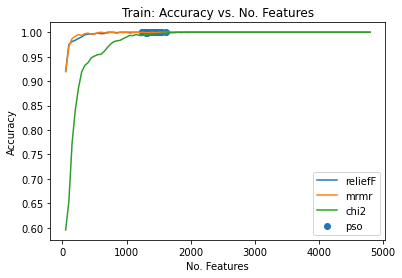
\includegraphics[width=\linewidth]{accuracy-features-fish-train.png}
    \caption{Species: Training set}\label{fig:accuracy-features-fish-train}
  \end{subfigure}
  \begin{subfigure}[b]{.45\linewidth}
    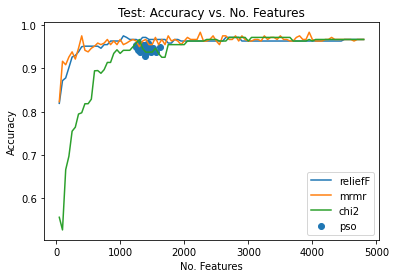
\includegraphics[width=\linewidth]{accuracy-features-fish-test.png}
    \caption{Species: Test set}\label{fig:accuracy-features-fish-test}
  \end{subfigure}
  \begin{subfigure}[b]{.45\linewidth}
    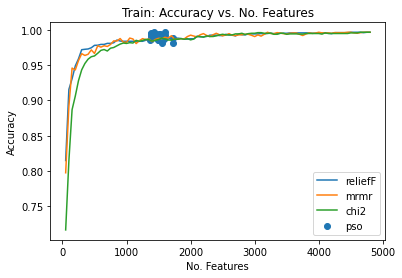
\includegraphics[width=\linewidth]{accuracy-features-part-train.png}
    \caption{Part: Training set}\label{fig:accuracy-features-part-train}
  \end{subfigure}
  \begin{subfigure}[b]{.45\linewidth}
    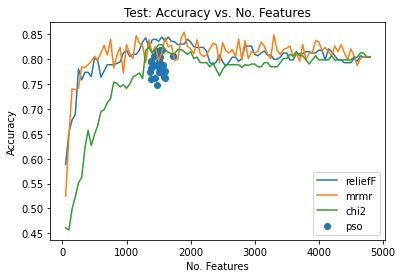
\includegraphics[width=\linewidth]{accuracy-features-part-test.png}
    \caption{Part: Test set}\label{fig:accuracy-features-part-test}
  \end{subfigure}
  \caption[Two numerical solutions]{
    Fish part dataset: classification accuracy for feature selection methods for a given $k$.
    Fish species dataset: Classification accuracy for feature selection methods for a given $k$.
    We measure the balanced accuracy of k-fold cross-validation.
    We compare reliefF, maximum relevance - minimum redundancy (MRMR), chi$^2$, and particle swarm optimisation (PSO).
    Fish part dataset. (a) Training set. (b) Test set.}
  \label{fig:animals}
\end{figure}

Figure~\ref{fig:accuracy-features-fish-train} shows accuracy for fish species.
We show accuracy on the training set for each feature selection method.
At $k=1050$ all feature selection methods achieve $100\%$ accuracy on the training set.
The SVM fits the training data for each method using a fraction of the full feature set.
Figure~\ref{fig:accuracy-features-fish-test} shows accuracy for fish species.
We show test set accuracy for each feature selection method.
The accuracy reaches a plateau ($96\%$ accuracy) at around $k=1050$ features for all methods.
The test performance is less than the train performance, yet the test accuracy is still very high.
This suggests the model can generalize well on unseen data for the fish species.

Figure~\ref{fig:accuracy-features-part-train} shows accuracy for part dataset.
We show train accuracy for each feature selection method.
All feature selection methods struggle to fit the training set for the fish part.
Even with the full feature set, a perfect train accuracy is never reached.
Figure~\ref{fig:accuracy-features-part-test} shows accuracy for part dataset.
We show the test accuracy for each feature selection method.
The classification accuracy fluctuates for all feature selection methods.
At around $k=1050$ features, it begins to decrease.
The training accuracy improves, as the test does not from this point onwards.
The SVM is overfitting to noise (redundant features) in the training set.

\subsection{Disucssion}
\label{sec:results-feature-selection-discussion}

Feature selection methods helped reduce dimensionality.
We evaluated performance with an SVM classifier.
In which, ReliefF and PSO were best for fish species and part, respectively.
ReliefF can identify conditional dependencies between features when providing feature rankings.
ReliefF algorithms are robust and noise-tolerant, which explains their superior performance.
PSO provides a combination of global and local searches.
A search through a near-infinite combinatorial space of possible feature subsets.
This stochastic method is computationally expensive but can offer effective solutions.

For both general and specific cases, and across all methods, the fish species have lower variance than the fish part in classification accuracy.
The classification results (\S~\ref{sec:results-classification}) support this, they also show higher test accuracy for fish species, than fish part.
They suggest different fish parts may have fewer underlying structural differences.

For the general case and both datasets, a lot of interesting behaviour happens at $k=1050$.
The fish species reach a plateau, but the fish part accuracy begins to decrease.
An accuracy comparable or better than the full dataset is possible with 21.8\% of its features.

For the fish species dataset, we see high accuracy with very few features.
ReliefF and MRMR can achieve above 90\% classification accuracy with $k = 50$.
Chi$^2$ is not able to mirror this performance.
This shows ReliefF and MRMR are very effective feature selection methods for this task.

The PSO may not have a hyperparameter for feature number $k$.
Instead, it automates the selection of this parameter.
Yet, it achieves comparable results to other state-of-the-art methods.
This automation may prove useful for automating the classification task for online learning.
In a factory, we may want to train a model as new data arrives.
PSO requires less human intervention, yet still, provides competitive performance.

MRMR and ReliefF both have high accuracy with very few features on the fish species dataset.
This suggests that few features are required to construct a reasonable representation of a fish tissue sample.
This is a good indication that the fish species dataset contains less noise.
This also warrants further investigation into which features are considered important for low $k$ values.
This motivates the following section on visualisation.

\section{Conclusions and Future Work}

% TODO [ ] - Summarize the achieved results to show the effectiveness of machine learning algorithms that were used. 

The analysis of fish oil data in this paper has focussed on interpretability. 
Not only have we found effective classification and feature selection techniques, but we have also tried to explain their performance with visualisation and analytical results. 
We can draw many conclusions from the analytical results and visualisations, but here we recall the most important:

\begin{enumerate}
  \item Fish species are easier to predict than fish part - there is more intra-class variation within fish species than there is a similarity between the same part from different fish.
  \item The Linear SVM classifier performs better for both classification tasks - the fish oil data is linearly separable on a hyperplane.
  \item Near-perfect accuracy can be achieved with very few features for fish species - if this predictive ability exceeds human error this model has real-world applications.
  \item Comparison with PSO may be difficult (due to automatic $k$ selection), but this automation may be useful in a factory setting.
\end{enumerate}

Feature selection is not guaranteed to improve classification accuracy.
Yet, it does reduce the complexity, increase interpretability and improve computational efficiency.
As with the SVM using an l1 regularization, feature selection is also a trade-off between interpretability and performance.
Arthur C. Clarke said, "[a]ny sufficiently advanced technology is indistinguishable from magic." \cite{clarke2013profiles}.
A perfect blackbox model is equivalent to magic, and, it is difficult to have faith in magic, especially if it were to be involved in our food making.
Faith isn't needed when our models when are interpretable.

% TODO [ ] - Future work: further steps, improve fish part performance, more challenging datasets, different tasks. 

% Please note that the first paragraph of a section or subsection is
% not indented. The first paragraph that follows a table, figure,
% equation etc. does not need an indent, either.

% Subsequent paragraphs, however, are indented.

% \subsubsection{Sample Heading (Third Level)} Only two levels of
% headings should be numbered. Lower level headings remain unnumbered;
% they are formatted as run-in headings.

% \paragraph{Sample Heading (Fourth Level)}
% The contribution should contain no more than four levels of
% headings. Table~\ref{tab1} gives a summary of all heading levels.

% \begin{table}
% \caption{Table captions should be placed above the
% tables.}\label{tab1}
% \begin{tabular}{|l|l|l|}
% \hline
% Heading level &  Example & Font size and style\\
% \hline
% Title (centered) &  {\Large\bfseries Lecture Notes} & 14 point, bold\\
% 1st-level heading &  {\large\bfseries 1 Introduction} & 12 point, bold\\
% 2nd-level heading & {\bfseries 2.1 Printing Area} & 10 point, bold\\
% 3rd-level heading & {\bfseries Run-in Heading in Bold.} Text follows & 10 point, bold\\
% 4th-level heading & {\itshape Lowest Level Heading.} Text follows & 10 point, italic\\
% \hline
% \end{tabular}
% \end{table}


% \noindent Displayed equations are centered and set on a separate
% line.
% \begin{equation}
% x + y = z
% \end{equation}
% Please try to avoid rasterized images for line-art diagrams and
% schemas. Whenever possible, use vector graphics instead (see
% Fig.~\ref{fig1}).

% \begin{figure}
% 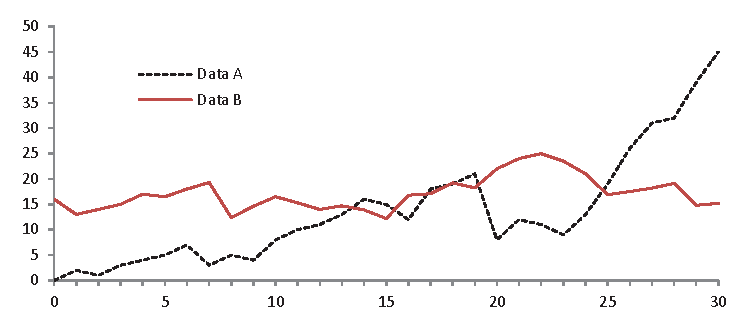
\includegraphics[width=\textwidth]{fig1.eps}
% \caption{A figure caption is always placed below the illustration.
% Please note that short captions are centered, while long ones are
% justified by the macro package automatically.} \label{fig1}
% \end{figure}

% \begin{theorem}
% This is a sample theorem. The run-in heading is set in bold, while
% the following text appears in italics. Definitions, lemmas,
% propositions, and corollaries are styled the same way.
% \end{theorem}
%
% the environments 'definition', 'lemma', 'proposition', 'corollary',
% 'remark', and 'example' are defined in the LLNCS documentclass as well.
%
% \begin{proof}
% Proofs, examples, and remarks have the initial word in italics,
% while the following text appears in normal font.
% \end{proof}
% For citations of references, we prefer the use of square brackets
% and consecutive numbers. Citations using labels or the author/year
% convention are also acceptable. The following bibliography provides
% a sample reference list with entries for journal
% articles~\cite{ref_article1}, an LNCS chapter~\cite{ref_lncs1}, a
% book~\cite{ref_book1}, proceedings without editors~\cite{ref_proc1},
% and a homepage~\cite{ref_url1}. Multiple citations are grouped
% \cite{ref_article1,ref_lncs1,ref_book1},
% \cite{ref_article1,ref_book1,ref_proc1,ref_url1}.
%
% ---- Bibliography ----
%
% BibTeX users should specify bibliography style 'splncs04'.
% References will then be sorted and formatted in the correct style.
%
\bibliographystyle{splncs04}
% \bibliography{mybibliography}
\bibliography{refs}

\end{document}
